% ============================================================
%  Présentation PFA – Commande Neuronale d'un Système Thermique à Distance
%  Beamer – visuel, centré sur les graphes
% ============================================================
\documentclass[aspectratio=169,12pt]{beamer}

% ---------- Encodage et langue ----------
\usepackage[utf8]{inputenc}
\usepackage[T1]{fontenc}
\usepackage[french]{babel}

% ---------- Packages ----------
\usepackage{amsmath,amssymb}
\usepackage{graphicx}
\usepackage{booktabs}
\usepackage{tikz}
\usetikzlibrary{arrows.meta,positioning,calc,shapes.geometric}
\usepackage{multicol}
\usepackage{xcolor}

% ---------- Thème ----------
\usetheme{Madrid}
\usecolortheme{whale}

% Couleurs ENIT
\definecolor{enitblue}{RGB}{0,51,102}
\definecolor{enitred}{RGB}{178,34,34}
\definecolor{enitgray}{RGB}{100,100,100}
\definecolor{lightblue}{RGB}{220,235,250}

\setbeamercolor{structure}{fg=enitblue}
\setbeamercolor{title}{fg=white,bg=enitblue}
\setbeamercolor{frametitle}{fg=white,bg=enitblue}
\setbeamercolor{block title}{bg=enitblue,fg=white}
\setbeamercolor{block body}{bg=lightblue,fg=black}
\setbeamercolor{item}{fg=enitblue}
\setbeamercolor{block title alerted}{bg=enitred,fg=white}
\setbeamercolor{block body alerted}{bg=enitred!8,fg=black}
\setbeamercolor{block title example}{bg=green!40!black,fg=white}
\setbeamercolor{block body example}{bg=green!5,fg=black}

\setbeamerfont{title}{size=\large,series=\bfseries}
\setbeamerfont{frametitle}{size=\normalsize,series=\bfseries}

% Footer
\setbeamertemplate{footline}{%
  \leavevmode%
  \hbox{%
    \begin{beamercolorbox}[wd=.333333\paperwidth,ht=2.5ex,dp=1ex,center]{author in head/foot}%
      \usebeamerfont{author in head/foot}\insertshortauthor
    \end{beamercolorbox}%
    \begin{beamercolorbox}[wd=.333333\paperwidth,ht=2.5ex,dp=1ex,center]{title in head/foot}%
      \usebeamerfont{title in head/foot}\insertshorttitle
    \end{beamercolorbox}%
    \begin{beamercolorbox}[wd=.333333\paperwidth,ht=2.5ex,dp=1ex,right]{date in head/foot}%
      \usebeamerfont{date in head/foot}\insertshortdate{}\hspace*{2em}
      \insertframenumber{} / \inserttotalframenumber\hspace*{2ex}
    \end{beamercolorbox}}%
  \vskip0pt%
}
\setbeamertemplate{navigation symbols}{}

% Chemin des figures
\graphicspath{{figures/}}

% ---------- Infos ----------
\title[Commande Neuronale]{Commande Neuronale d'un Système Thermique à Distance}
\subtitle{Projet de Fin d'Année~II}
\author[Ouri \& Chaanbi]{Ouri Mohamed Amine \and Chaanbi Hassen}
\institute[ENIT]{ENIT -- Département Génie Électrique}
\date{2025/2026}

% ============================================================
\begin{document}

% ============================================================
% SLIDE 1 : Page de garde
% ============================================================
{
\setbeamertemplate{footline}{}
\begin{frame}[plain]
\begin{tikzpicture}[remember picture,overlay]
  \fill[enitblue] (current page.north west) rectangle (current page.south east);
  \fill[white,opacity=0.92] ([yshift=-2.5cm]current page.north west) rectangle (current page.south east);
  \node[anchor=north,text=white,font=\small] at ([yshift=-0.4cm]current page.north) {
    République Tunisienne -- Ministère de l'Enseignement Supérieur et de la Recherche Scientifique
  };
  \node[anchor=north,text=white,font=\small] at ([yshift=-1.0cm]current page.north) {
    Université de Tunis El Manar -- École Nationale d'Ingénieurs de Tunis
  };
  \node[anchor=north,text=white,font=\small] at ([yshift=-1.6cm]current page.north) {
    Département Génie Électrique
  };
\end{tikzpicture}

\vspace{2.0cm}
\begin{center}
  {\color{enitblue}\large\textbf{PROJET DE FIN D'ANNÉE~II}}\\[12pt]
  {\color{enitblue}\LARGE\textbf{Commande Neuronale d'un}}\\[4pt]
  {\color{enitblue}\LARGE\textbf{Système Thermique à Distance}}\\[20pt]
  {\color{enitgray}\rule{0.4\textwidth}{0.5pt}}\\[12pt]
  \begin{tabular}{rl}
    \textbf{Réalisé par :} & Ouri Mohamed Amine \\
                           & Chaanbi Hassen \\[6pt]
    \textbf{Encadré par :} & Mr. Bouani Faouzi \\[6pt]
    \textbf{Filière :}     & 2\textsuperscript{ème} Année GE~2
  \end{tabular}\\[16pt]
  {\color{enitgray}\small Année universitaire : 2025/2026}
\end{center}
\end{frame}
}

% ============================================================
% SLIDE 2 : Plan
% ============================================================
\begin{frame}{Plan de la présentation}
\tableofcontents
\end{frame}

% ============================================================
\section{Problématique et objectifs}
% ============================================================

% SLIDE 3
\begin{frame}{Problématique}
\begin{columns}[c]
\column{0.55\textwidth}
\begin{alertblock}{Le problème}
Comment commander un système thermique \textbf{non linéaire} dont le modèle est \textbf{inconnu}, \textbf{à distance} ?
\end{alertblock}

\vspace{4pt}
\begin{itemize}
  \item PID $\rightarrow$ nécessite un modèle connu
  \item Systèmes réels $\rightarrow$ non linéaires, perturbés
  \item Solution $\rightarrow$ \textbf{réseaux de neurones}
\end{itemize}

\column{0.4\textwidth}
\begin{center}
\begin{tikzpicture}[scale=0.7, every node/.style={font=\footnotesize},
  block/.style={draw, rounded corners, minimum height=9mm, minimum width=22mm, fill=lightblue, align=center}]
  \node[block, fill=enitred!15] (pid) at (0,2) {PID\\{\tiny modèle requis}};
  \node[block, fill=green!15] (nn) at (0,0) {Neurone\\{\tiny sans modèle}};
  \node[block] (sys) at (0,-2) {Système\\thermique};
  \draw[-Stealth, dashed, enitred] (pid) -- (sys) node[midway, right]{\tiny\color{enitred} limité};
  \draw[-Stealth, thick, green!50!black] (nn) -- (sys) node[midway, right]{\tiny\color{green!50!black} adapté};
\end{tikzpicture}
\end{center}
\end{columns}
\end{frame}

% SLIDE 4
\begin{frame}{Objectifs et démarche}
\begin{center}
\begin{tikzpicture}[scale=0.9, every node/.style={font=\small},
  phase/.style={draw=enitblue, rounded corners=6pt, fill=lightblue, 
    minimum height=14mm, minimum width=35mm, align=center, font=\small\bfseries}]
  \node[phase] (p1) at (0,0) {Théorie};
  \node[phase] (p2) at (5,0) {Simulation\\Matlab};
  \node[phase] (p3) at (10,0) {Implémentation\\ESP32};
  \draw[-Stealth, thick, enitblue] (p1) -- (p2);
  \draw[-Stealth, thick, enitblue] (p2) -- (p3);
  
  \node[font=\footnotesize, text=enitgray, below=3mm] at (p1.south) {Ch.~1};
  \node[font=\footnotesize, text=enitgray, below=3mm] at (p2.south) {Ch.~2};
  \node[font=\footnotesize, text=enitgray, below=3mm] at (p3.south) {Ch.~3};
\end{tikzpicture}
\end{center}

\vspace{10pt}
\begin{columns}[t]
\column{0.3\textwidth}
\begin{itemize}\small
  \item PID vs Neuronale
  \item Fondements MLP
\end{itemize}
\column{0.3\textwidth}
\begin{itemize}\small
  \item PID sur syst. linéaire
  \item Identification neuronale
  \item Commande min. variance
\end{itemize}
\column{0.3\textwidth}
\begin{itemize}\small
  \item Boucle ouverte / fermée
  \item Communication sans fil
  \item Validation expérimentale
\end{itemize}
\end{columns}
\end{frame}

% ============================================================
\section{Fondements théoriques}
% ============================================================

% SLIDE 5
\begin{frame}{Neurone artificiel et MLP}
\begin{columns}[c]
\column{0.45\textwidth}
\begin{center}
\begin{tikzpicture}[scale=0.85, every node/.style={font=\small}]
  \foreach \i/\label in {1/x_1, 2/x_2, 3/x_n} {
    \node[circle, draw, minimum size=6mm] (I\i) at (0, -\i*1.2+0.6) {$\label$};
  }
  \node at (0, -1.8) {$\vdots$};
  \node[circle, draw=enitblue, fill=lightblue, minimum size=12mm] (N) at (3, -1.2) {$\Sigma$};
  \node[rectangle, draw=enitred, fill=enitred!10, minimum height=8mm, minimum width=10mm] (A) at (5, -1.2) {$\varphi$};
  \node (O) at (6.8, -1.2) {$y$};
  \draw[-Stealth] (I1) -- node[above,font=\tiny]{$w_1$} (N);
  \draw[-Stealth] (I2) -- node[above,font=\tiny]{$w_2$} (N);
  \draw[-Stealth] (I3) -- node[below,font=\tiny]{$w_n$} (N);
  \draw[-Stealth] (N) -- (A);
  \draw[-Stealth] (A) -- (O);
  \node (B) at (3, 0.6) {$b$};
  \draw[-Stealth] (B) -- (N);
\end{tikzpicture}
\end{center}

\vspace{4pt}
$$y = \varphi\!\left(\sum_{i=0}^{n} w_i x_i\right)$$

\column{0.5\textwidth}
\textbf{Fonctions d'activation :}
\begin{itemize}\small
  \item Sigmoïde : $\sigma(v) = \frac{1}{1+e^{-v}} \in [0,1]$
  \item Tanh : $\tanh(v) \in (-1,1)$
\end{itemize}

\vspace{6pt}
\textbf{MLP -- propagation avant :}
$$\mathbf{a}^{(\ell)} = \varphi\!\left(W^{(\ell)}\mathbf{a}^{(\ell-1)} + \mathbf{b}^{(\ell)}\right)$$

\vspace{4pt}
\begin{exampleblock}{\small Théorème (Cybenko, 1989)}
\small Un MLP à 1 couche cachée approxime toute fonction continue.
\end{exampleblock}
\end{columns}
\end{frame}

% SLIDE 6
\begin{frame}{Commande neuronale d'un système inconnu}
\begin{columns}[c]
\column{0.5\textwidth}
\begin{center}
\begin{tikzpicture}[scale=0.85, every node/.style={font=\small},
  block/.style={draw, rounded corners, minimum height=10mm, minimum width=22mm, fill=lightblue, font=\small\bfseries}]
  \node[block] (ctrl) at (0,0) {Contrôleur\\{\tiny (neurone)}};
  \node[block, fill=enitred!12] (sys) at (4.5,0) {Système\\{\tiny (inconnu)}};
  \node (r) at (-2.8,0) {$r(t)$};
  \node (y) at (7.3,0) {$y(t)$};
  \node[circle,draw,inner sep=1.5pt] (sum) at (-1.4, 0) {\tiny$+$};
  \draw[-Stealth] (r) -- (sum);
  \draw[-Stealth] (sum) -- (ctrl);
  \draw[-Stealth] (ctrl) -- node[above]{\small$u$} (sys);
  \draw[-Stealth] (sys) -- (y);
  \draw[-Stealth] (6.3,0) -- (6.3,-1.3) -- (-1.4,-1.3) -- (sum);
  \node at (-1.1,-0.95) {\tiny$-$};
\end{tikzpicture}
\end{center}

\column{0.45\textwidth}
\textbf{2 étapes :}
\begin{enumerate}\small
  \item \textbf{Identification} : le MLP apprend $\hat{y} = f(u, y_{\text{passé}})$
  \item \textbf{Commande} : minimiser $e = r - y$
\end{enumerate}

\vspace{6pt}
\textbf{Apprentissage} (descente de gradient) :
$$\Theta \leftarrow \Theta - \mu\,\nabla\mathcal{L}$$
$$\mathcal{L} = \frac{1}{N}\sum_{k}|y^{(k)} - \hat{y}^{(k)}|^2$$
\end{columns}
\end{frame}

% ============================================================
\section{Simulation et analyse}
% ============================================================

% SLIDE 7
\begin{frame}{Simulation PID -- Réponse en boucle ouverte}
\begin{columns}[c]
\column{.55\textwidth}
\begin{center}
  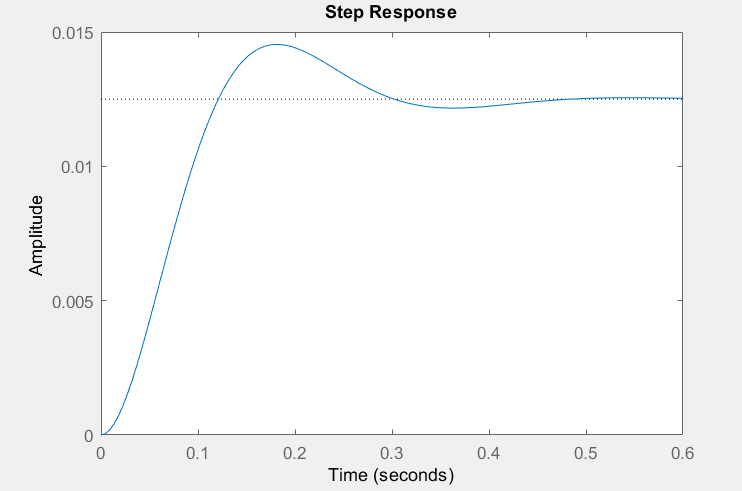
\includegraphics[width=\linewidth]{fig_p26_1.png}
\end{center}
\vspace{-4pt}
{\footnotesize\centering Réponse indicielle -- boucle ouverte ($\xi=0{,}5$ : sous-amorti)\par}

\column{0.4\textwidth}
\small
$H(s) = \dfrac{K_s\omega_0^2}{s^2+2\xi\omega_0 s+\omega_0^2}$

\vspace{6pt}
\begin{tabular}{lc}
  \toprule
  $K_s$ & 5 \\
  $\omega_0$ & 20 rad/s \\
  $\xi$ & 0,5 \\
  $T_e$ & 0,36 s \\
  \bottomrule
\end{tabular}

\vspace{8pt}
{\footnotesize Dépassement visible $\Rightarrow$ besoin d'un correcteur.}
\end{columns}
\end{frame}

% SLIDE 8
\begin{frame}{Simulation PID -- Résultats en boucle fermée}
\begin{center}
  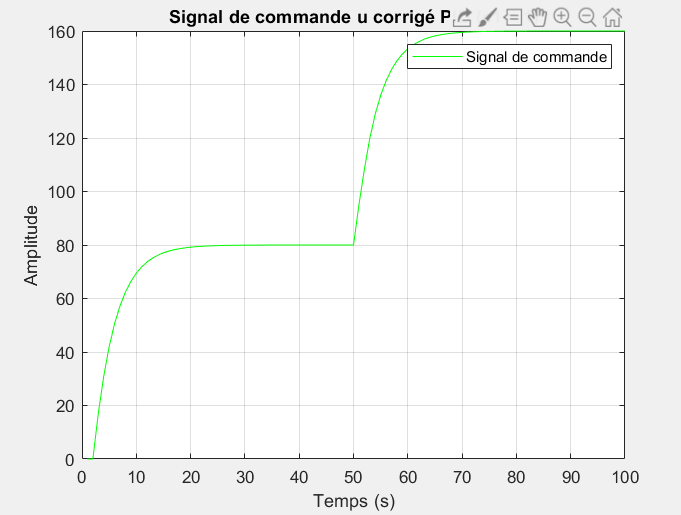
\includegraphics[height=0.55\textheight]{fig_p27_1.png}\hfill
  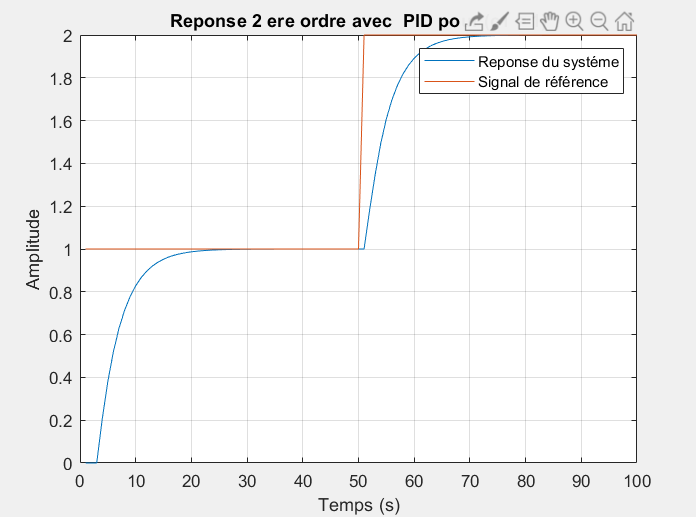
\includegraphics[height=0.55\textheight]{fig_p27_2.png}
\end{center}
\vspace{-2pt}
{\footnotesize\centering (a) Signal de commande $u(k)$ \hspace{3cm} (b) Réponse $y(k)$ avec PID\par}

\vspace{4pt}
\begin{center}
\small $c_0=15,\; c_1=1,\; c_2=1 \;\Rightarrow\; K_p=-3,\; K_i\approx47{,}2,\; K_d=0{,}36$
\quad\textbar\quad \textbf{Suivi correct, erreur statique nulle}
\end{center}
\end{frame}

% SLIDE 9
\begin{frame}{Identification neuronale -- Système non linéaire}
\begin{block}{}
\small $y(k) = -0{,}8\, y(k\!-\!2)\,\dfrac{[u(k\!-\!1)]^2}{1+[u(k\!-\!1)]^2} + 0{,}033\, y(k\!-\!1) + 0{,}5\, u(k\!-\!1)$
\end{block}

\vspace{2pt}
\begin{columns}[c]
\column{0.48\textwidth}
\begin{center}
  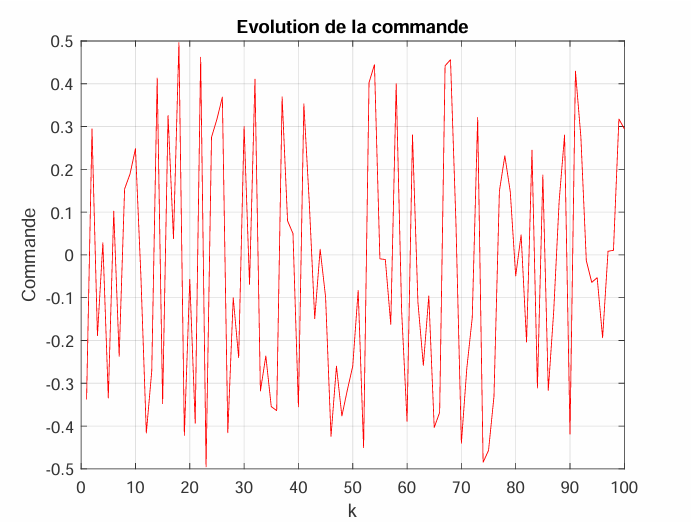
\includegraphics[width=\linewidth]{fig_p29_1.png}
\end{center}
\vspace{-4pt}
{\footnotesize\centering Commande aléatoire $u(k)\in[-0{,}5;\,0{,}5]$\par}

\column{0.48\textwidth}
\small
\textbf{Topologie :}
\begin{itemize}\footnotesize
  \item Entrées : $[-1,\; u(k\!-\!1),\; y(k\!-\!1)]^\top$
  \item Sortie : $\hat{y}(k) = \tanh(\mathbf{w}^\top\mathbf{x})$
\end{itemize}
\vspace{4pt}
Non-linéarité + mémoire $(k\!-\!1, k\!-\!2)$
\end{columns}
\end{frame}

% SLIDE 10
\begin{frame}{Résultats de l'identification neuronale}
\begin{center}
  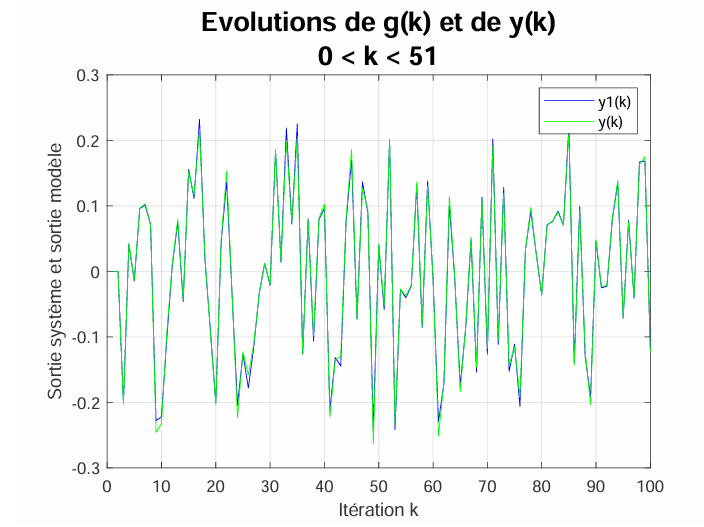
\includegraphics[height=0.42\textheight]{fig_p29_2.png}\hfill
  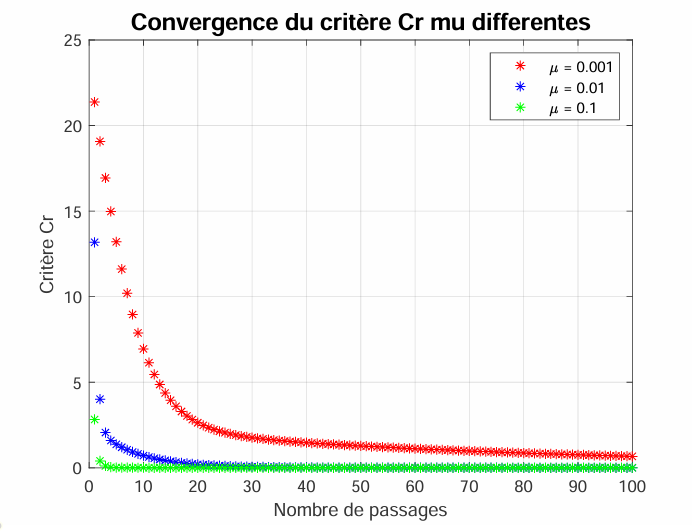
\includegraphics[height=0.42\textheight]{fig_p29_3.png}
\end{center}
\vspace{-2pt}
{\footnotesize\centering (a) $y(k)$ vs $\hat{y}(k)$ \hspace{4cm} (b) Convergence du critère $C_r$ pour différents $\mu$\par}

\vspace{6pt}
\begin{center}
\small
\begin{tabular}{ccc}
  \toprule
  $\mu$ & Comportement & Verdict \\
  \midrule
  0,001 & Très lent & Trop lent \\
  \textbf{0,01} & \textbf{Régulier} & \textbf{Optimal} \\
  0,1 & Rapide & Risque d'oscillations \\
  \bottomrule
\end{tabular}
\end{center}
\end{frame}

% SLIDE 11
\begin{frame}{Commande par minimum de variance -- Principe}
\begin{columns}[c]
\column{0.55\textwidth}
\textbf{Critère :}
$$J = \left[y_c(k\!+\!1) - \hat{y}(k\!+\!1)\right]^2 + \lambda\left[u(k) - u(k\!-\!1)\right]^2$$

\vspace{4pt}
\textbf{Optimisation itérative} ($i_{\max}=10$) :
$$u_{\text{new}} = u_{\text{old}} - \mu\,\frac{\partial J}{\partial u}, \quad \mu = 0{,}2$$

\vspace{4pt}
{\small $\lambda$ petit $\Rightarrow$ rapide \quad\textbar\quad $\lambda$ grand $\Rightarrow$ lent}

\column{0.42\textwidth}
\begin{center}
  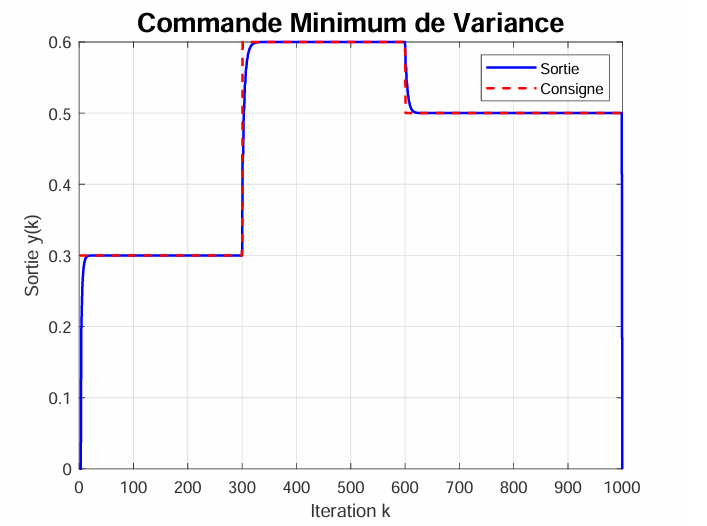
\includegraphics[width=\linewidth]{fig_p31_1.png}
\end{center}
\vspace{-4pt}
{\footnotesize\centering Suivi de consigne ($\lambda$ faible)\par}
\end{columns}
\end{frame}

% SLIDE 12
\begin{frame}{Commande min. variance -- Résultats}
\begin{center}
  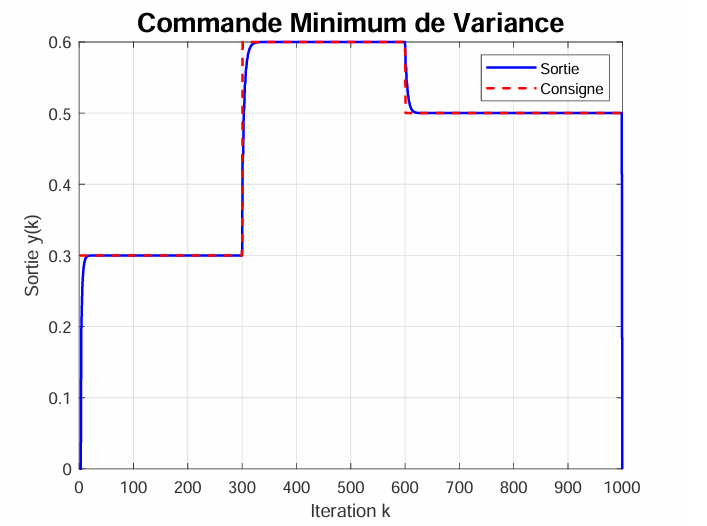
\includegraphics[height=0.42\textheight]{fig_p31_1.png}\hfill
  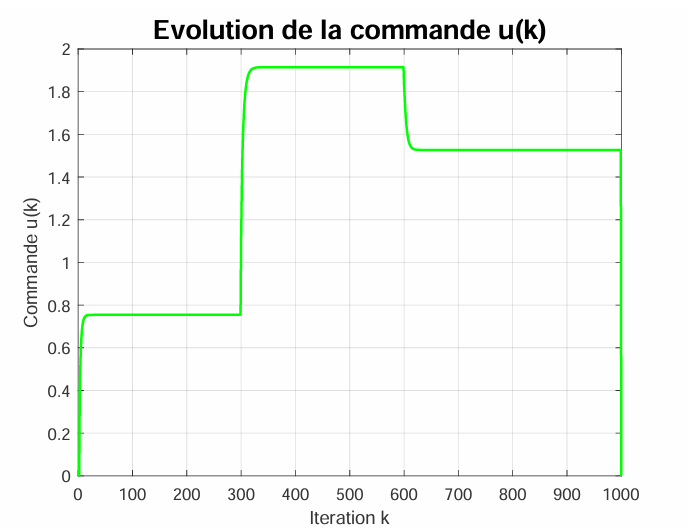
\includegraphics[height=0.42\textheight]{fig_p31_2.png}
\end{center}
\vspace{-2pt}
{\footnotesize\centering (a) Suivi de consigne ($\lambda$ faible) \hspace{2.5cm} (b) Signal de commande $u(k)$\par}

\vspace{4pt}
\begin{center}
  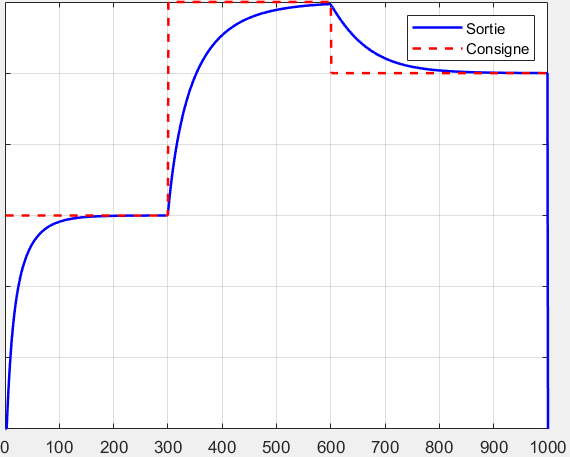
\includegraphics[height=0.28\textheight]{fig_p32_1.png}\hfill
  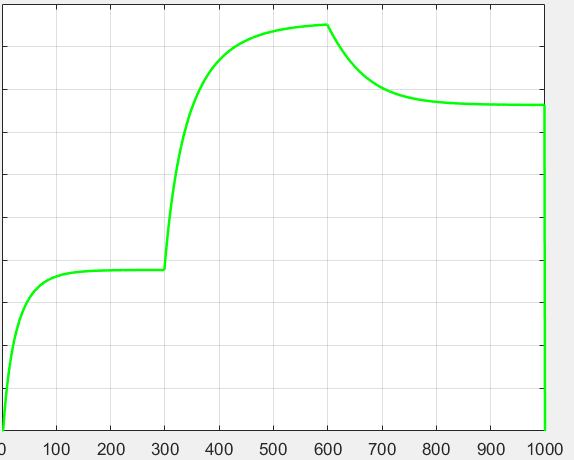
\includegraphics[height=0.28\textheight]{fig_p32_2.png}
\end{center}
\vspace{-2pt}
{\footnotesize\centering (c) $\lambda = 4$ : suivi dégradé \hspace{3cm} (d) Commande avec $\lambda = 4$\par}
\end{frame}

% SLIDE 13
\begin{frame}{Bilan des simulations}
\begin{columns}[c]
\column{0.48\textwidth}
\begin{block}{PID classique}
\begin{itemize}\small
  \item[\checkmark] Suivi correct (syst. linéaire)
  \item[\checkmark] Erreur statique nulle
  \item[$\times$] Modèle requis
  \item[$\times$] Inadapté au non linéaire
\end{itemize}
\end{block}

\column{0.48\textwidth}
\begin{exampleblock}{Commande neuronale}
\begin{itemize}\small
  \item[\checkmark] Pas de modèle requis
  \item[\checkmark] Identification efficace
  \item[\checkmark] Bon suivi de consigne
  \item[\checkmark] Adapté au non linéaire
\end{itemize}
\end{exampleblock}
\end{columns}

\vspace{10pt}
\begin{center}
\large $\Rightarrow$ \textbf{Passage à l'implémentation pratique}
\end{center}
\end{frame}

% ============================================================
\section{Implémentation pratique}
% ============================================================

% SLIDE 14
\begin{frame}{Composants matériels}
\begin{columns}[c]
\column{0.3\textwidth}
\begin{center}
  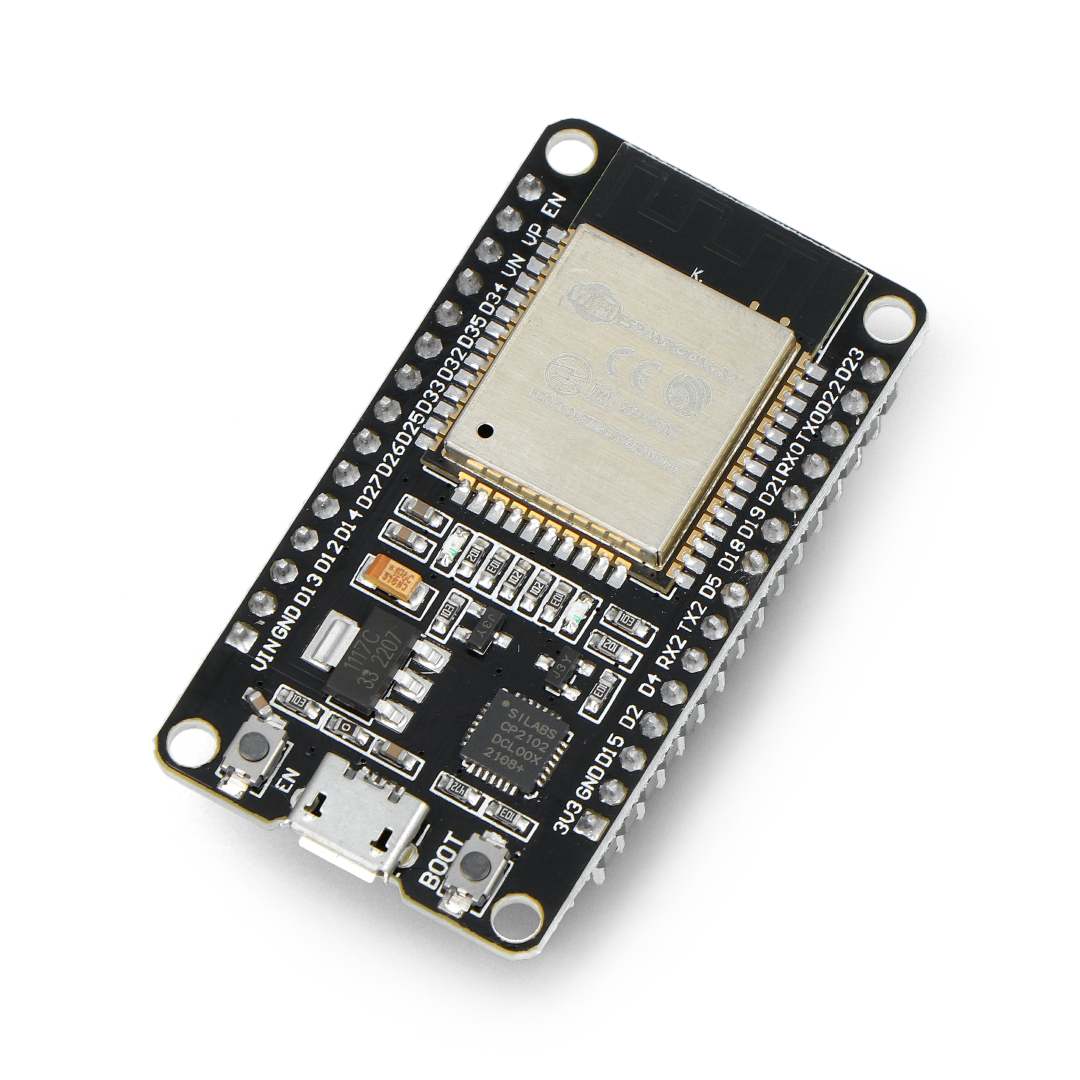
\includegraphics[width=0.85\linewidth]{fig_p34_1.jpeg}\\[2pt]
  {\footnotesize ESP32}
\end{center}

\column{0.3\textwidth}
\begin{center}
  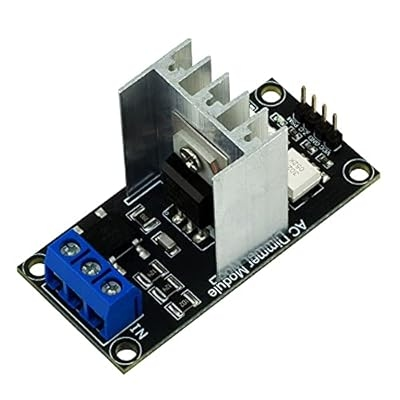
\includegraphics[width=0.7\linewidth]{fig_p36_1.jpeg}\\[2pt]
  {\footnotesize AC Dimmer}
\end{center}

\column{0.3\textwidth}
\begin{center}
  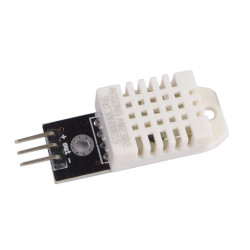
\includegraphics[width=0.65\linewidth]{fig_p36_2.jpeg}\\[2pt]
  {\footnotesize Capteur DHT22}
\end{center}
\end{columns}

\vspace{8pt}
\begin{center}
\small
\begin{tabular}{lccc}
  \toprule
  & \textbf{ESP32} & \textbf{Dimmer} & \textbf{DHT22} \\
  \midrule
  Rôle & Calcul \& comm. & Puissance AC & Mesure temp. \\
  Précision & -- & 8A, 220V & $\pm 0{,}1$°C \\
  \bottomrule
\end{tabular}
\end{center}
\end{frame}

% SLIDE 15
\begin{frame}{Architecture du système}
\begin{center}
\begin{tikzpicture}[scale=0.85, every node/.style={font=\small},
  block/.style={draw, rounded corners=4pt, minimum height=13mm, minimum width=30mm, 
    fill=lightblue, text=enitblue, font=\small\bfseries, align=center},
  hw/.style={draw, rounded corners=4pt, minimum height=13mm, minimum width=28mm, 
    fill=enitblue!8, font=\small, align=center}]
  
  \node[block, fill=enitred!15, text=enitred, minimum width=38mm] (box) at (0,0) {Boîte fermée\\{\tiny (enceinte thermique)}};
  \node[hw] (dht) at (-5, 0) {DHT22\\{\tiny capteur}};
  \node[hw] (lamp) at (5, 0) {Lampe 220V\\{\tiny source chaleur}};
  \node[block] (esp1) at (-5, -2.5) {ESP32\\mesure};
  \node[block] (esp2) at (5, -2.5) {ESP32\\commande};
  \node[hw] (dimmer) at (5, -4.8) {AC Dimmer};
  
  \draw[-Stealth, thick] (dht) -- (box);
  \draw[-Stealth, thick, enitred] (lamp) -- (box);
  \draw[-Stealth, thick] (dht) -- (esp1) node[midway, left]{\footnotesize temp.};
  \draw[Stealth-Stealth, ultra thick, enitblue, dashed] (esp1) -- (esp2) 
    node[midway, below=2pt]{\footnotesize\textbf{ESP-NOW} (sans fil, 2.4~GHz)};
  \draw[-Stealth, thick] (esp2) -- (dimmer) node[midway, right]{\footnotesize PWM};
  \draw[-Stealth, thick] (dimmer) -| (lamp) node[near start, right]{\footnotesize puissance};
\end{tikzpicture}
\end{center}
\end{frame}

% SLIDE 16
\begin{frame}{Essai en boucle ouverte -- Collecte de données}
\begin{columns}[c]
\column{0.48\textwidth}
\begin{center}
  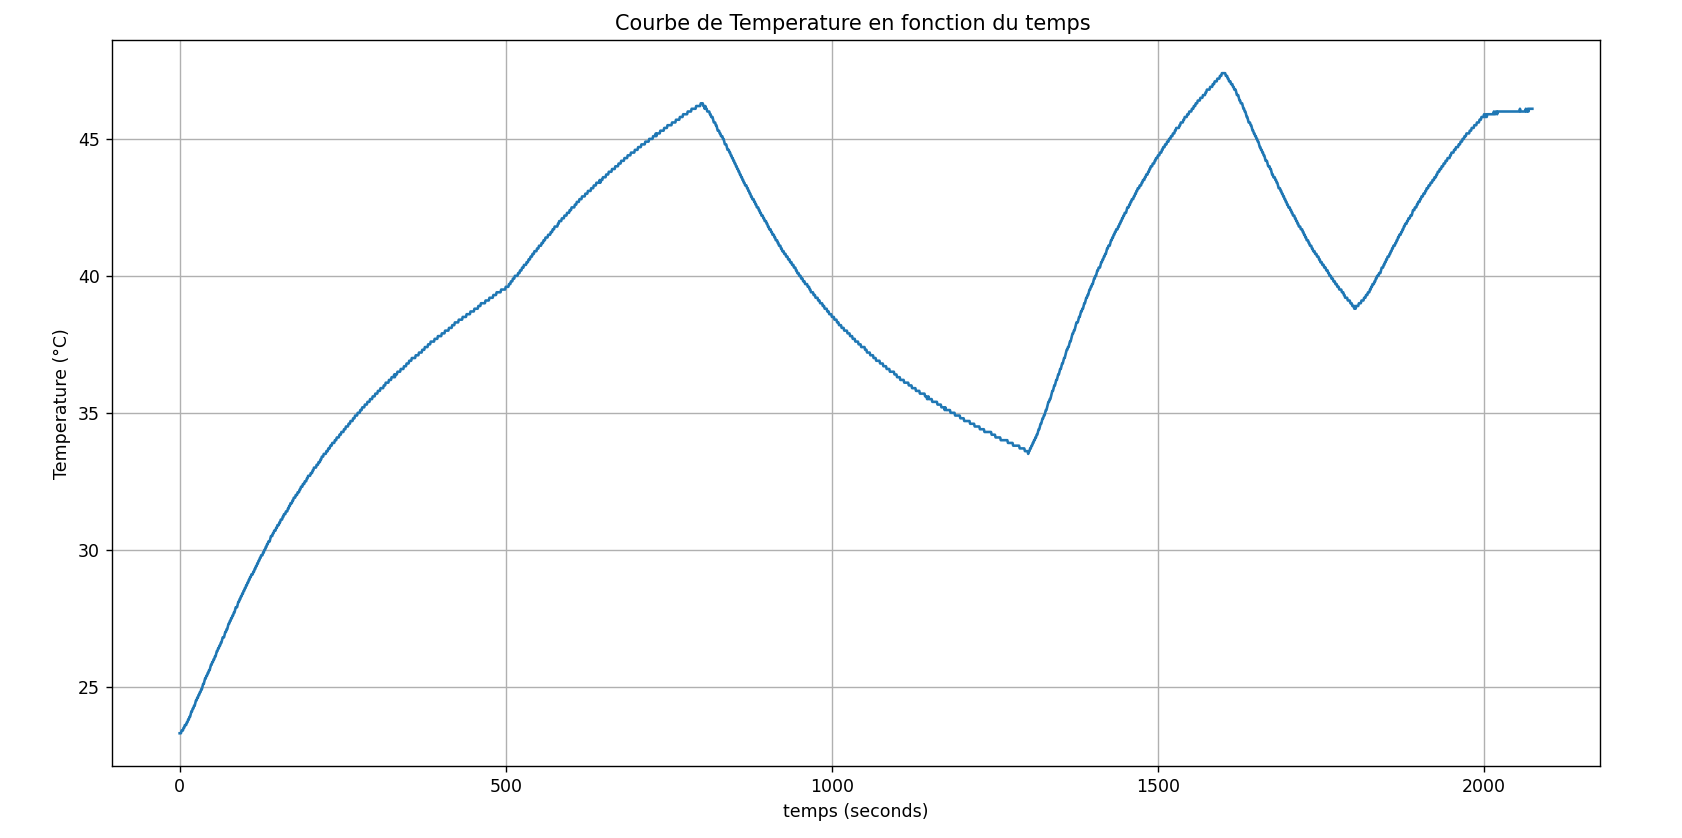
\includegraphics[width=\linewidth]{fig_p38_1.png}
\end{center}
\vspace{-4pt}
{\footnotesize\centering Température en fonction du temps\par}

\column{0.48\textwidth}
\begin{center}
  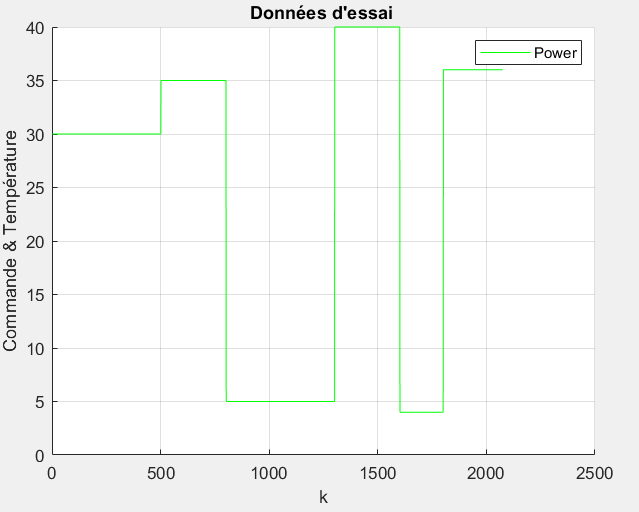
\includegraphics[width=\linewidth]{fig_p39_1.png}
\end{center}
\vspace{-4pt}
{\footnotesize\centering Commande appliquée\par}
\end{columns}

\vspace{6pt}
\begin{center}
\small Commande constante $u$ sur 2000 échantillons \quad\textbar\quad Échantillonnage : 2~s \quad\textbar\quad $\Rightarrow$ \textbf{Base d'apprentissage}
\end{center}
\end{frame}

% SLIDE 17
\begin{frame}{Apprentissage du neurone -- Phase d'entraînement}
\begin{center}
  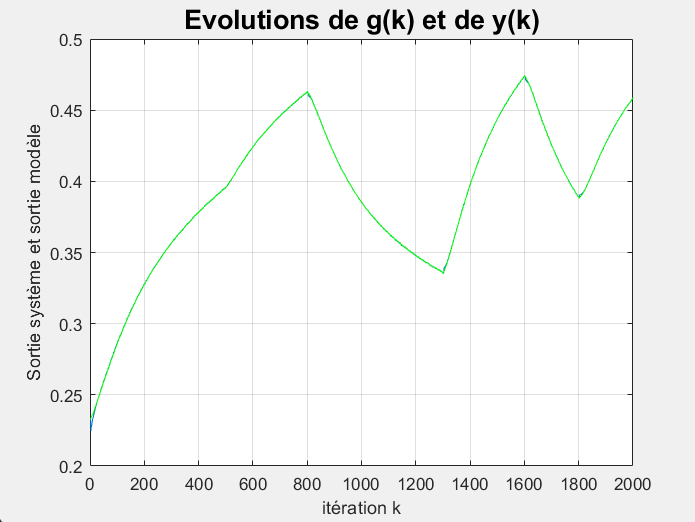
\includegraphics[height=0.65\textheight]{fig_p40_1.png}
\end{center}
\vspace{-4pt}
{\footnotesize\centering Sortie système vs sortie prédite du neurone -- \textbf{Phase d'apprentissage}\par}

\vspace{4pt}
\begin{center}
\small Données normalisées ($T/100$, $u/5$) \quad\textbar\quad Descente de gradient itérative
\end{center}
\end{frame}

% SLIDE 18
\begin{frame}{Apprentissage du neurone -- Phase de test}
\begin{center}
  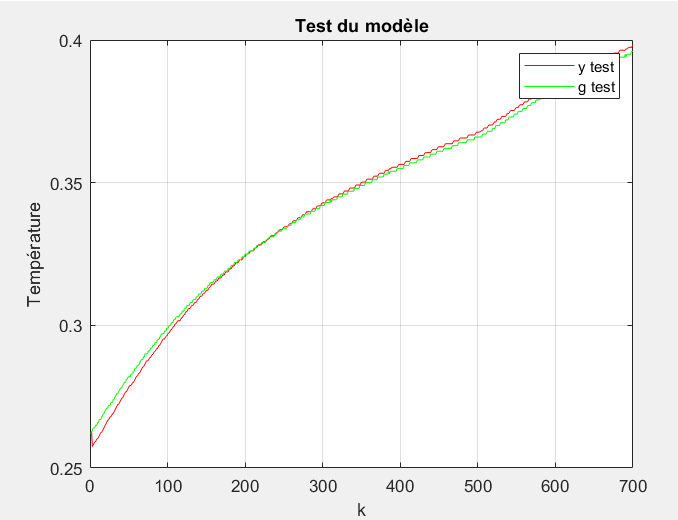
\includegraphics[height=0.65\textheight]{fig_p40_2.png}
\end{center}
\vspace{-4pt}
{\footnotesize\centering Sortie système vs sortie prédite du neurone -- \textbf{Phase de test}\par}

\vspace{4pt}
\begin{center}
\small Le modèle \textbf{généralise correctement} sur des données non vues $\Rightarrow$ poids validés
\end{center}
\end{frame}

% SLIDE 19
\begin{frame}{Montage expérimental -- Boucle fermée}
\begin{center}
  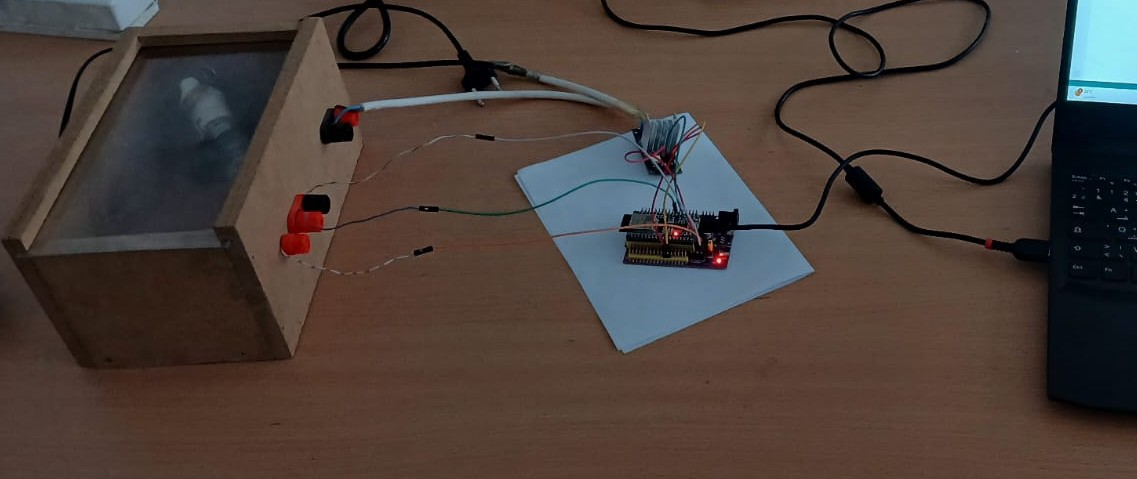
\includegraphics[height=0.7\textheight]{fig_p42_1.jpeg}
\end{center}
\vspace{-4pt}
{\footnotesize\centering Montage : ESP32 + Dimmer + DHT22 + Lampe + Boîte fermée\par}
\end{frame}

% SLIDE 20
\begin{frame}{Résultats en boucle fermée -- Commande câblée}
\begin{center}
  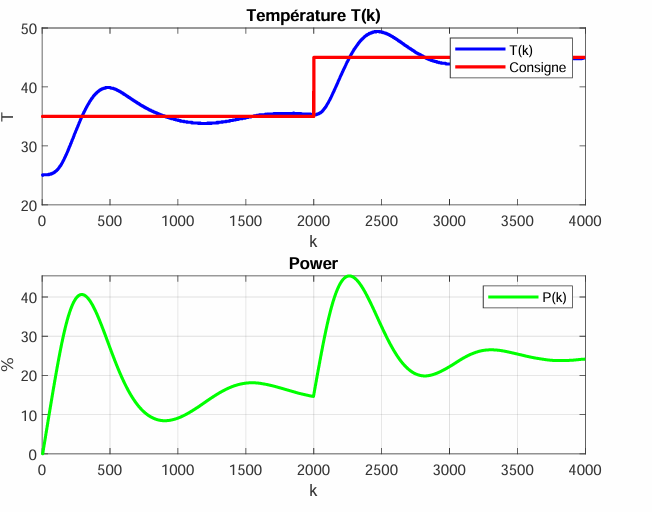
\includegraphics[height=0.62\textheight]{fig_p43_1.png}
\end{center}
\vspace{-4pt}
{\footnotesize\centering Consigne 35°C puis 45°C -- 4000 échantillons -- Échantillonnage 2~s\par}

\vspace{4pt}
\begin{center}
\small \textbf{La température suit la consigne} \quad\textbar\quad Oscillations faibles \quad\textbar\quad Système stable
\end{center}
\end{frame}

% ============================================================
\section{Communication sans fil}
% ============================================================

% SLIDE 21
\begin{frame}{Protocole ESP-NOW}
\begin{columns}[c]
\column{0.45\textwidth}
\begin{center}
\begin{tikzpicture}[scale=0.8, every node/.style={font=\footnotesize},
  card/.style={draw=enitblue, rounded corners=6pt, fill=lightblue, 
    minimum height=18mm, minimum width=30mm, align=center, font=\small\bfseries}]
  \node[card] (e1) at (0,0) {ESP32\\Commande};
  \node[card] (e2) at (5.5,0) {ESP32\\Mesure};
  \draw[-Stealth, ultra thick, enitred] ([yshift=3mm]e1.east) -- node[above]{\small Power (\%)} ([yshift=3mm]e2.west);
  \draw[-Stealth, ultra thick, enitblue] ([yshift=-3mm]e2.west) -- node[below]{\small Temp. (°C)} ([yshift=-3mm]e1.east);
  \node at (2.75, -1.5) {\small\textbf{2.4 GHz -- sans Wi-Fi}};
\end{tikzpicture}
\end{center}

\column{0.45\textwidth}
\begin{tabular}{ll}
  \toprule
  Fréquence & 2,4 GHz \\
  Latence & $\sim$ ms \\
  Portée & $\sim 200$ m \\
  Wi-Fi requis & Non \\
  Données max & 250 oct/trame \\
  \bottomrule
\end{tabular}
\end{columns}
\end{frame}

% SLIDE 22
\begin{frame}{Montage avec communication sans fil}
\begin{center}
  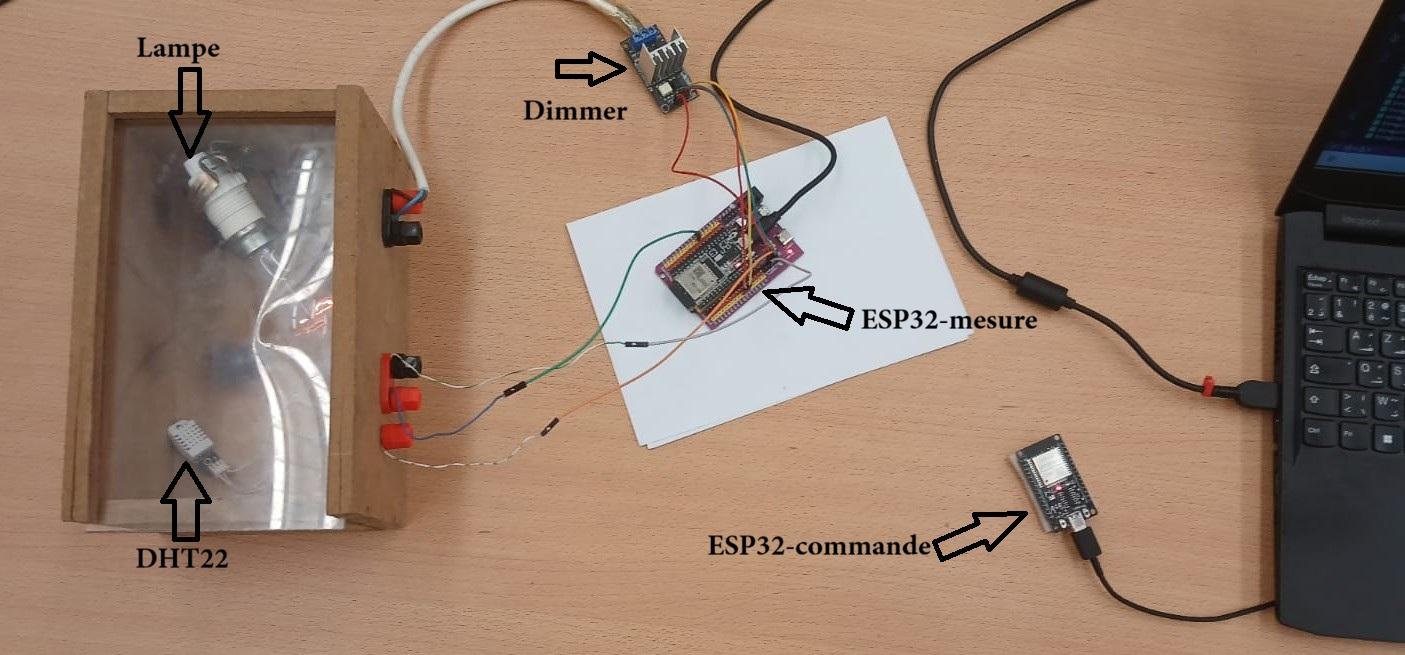
\includegraphics[height=0.7\textheight]{fig_p46_1.jpeg}
\end{center}
\vspace{-4pt}
{\footnotesize\centering Montage expérimental avec 2 cartes ESP32 communicant via ESP-NOW\par}
\end{frame}

% SLIDE 23
\begin{frame}{Résultats -- Commande à distance}
\begin{center}
  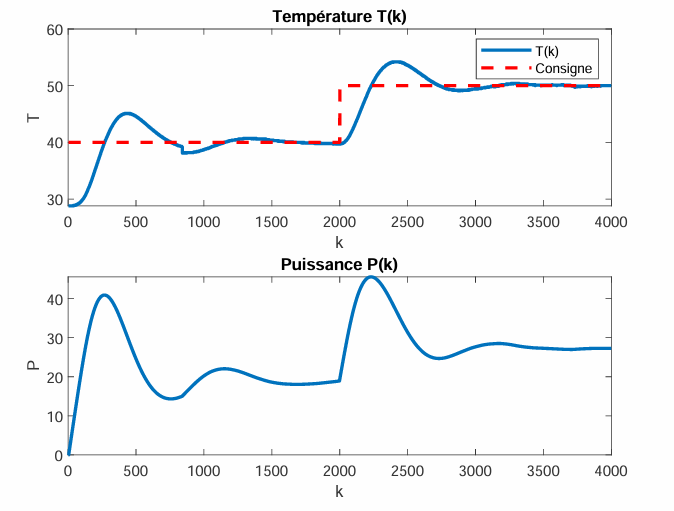
\includegraphics[height=0.62\textheight]{fig_p47_1.png}
\end{center}
\vspace{-4pt}
{\footnotesize\centering Consignes : 40°C puis 50°C -- Communication sans fil ESP-NOW\par}

\vspace{4pt}
\begin{center}
\small \textbf{Suivi de consigne confirmé} \quad\textbar\quad Retard dû à l'inertie thermique \quad\textbar\quad \textbf{Système stable}
\end{center}
\end{frame}

% ============================================================
\section{Bilan et conclusion}
% ============================================================

% SLIDE 24
\begin{frame}{Bilan comparatif}
\begin{center}
\begin{tabular}{p{3.2cm}p{4cm}p{4.5cm}}
  \toprule
  \textbf{Critère} & \textbf{PID classique} & \textbf{Commande neuronale} \\
  \midrule
  Modèle requis & Oui (obligatoire) & \textbf{Non} \\
  Syst. linéaires & Très efficace & Efficace \\
  Syst. non linéaires & Inadapté & \textbf{Adapté} \\
  Réglage & Manuel & Automatique \\
  Adaptabilité & Faible & \textbf{Forte} \\
  \bottomrule
\end{tabular}
\end{center}

\vspace{10pt}
\begin{exampleblock}{Conclusion clé}
\centering La commande neuronale est \textbf{complémentaire} au PID et \textbf{indispensable} pour les systèmes à modèle inconnu.
\end{exampleblock}
\end{frame}

% SLIDE 25
\begin{frame}{Conclusion}
\begin{columns}[c]
\column{0.48\textwidth}
\textbf{Ce qu'on a fait :}
\begin{enumerate}\small
  \item Fondements théoriques (PID vs RNA)
  \item Simulations Matlab validées
  \item Implémentation sur ESP32
  \item Communication sans fil ESP-NOW
  \item Validation expérimentale réussie
\end{enumerate}

\column{0.48\textwidth}
\textbf{Perspectives :}
\begin{itemize}\small
  \item MLP multicouche plus profond
  \item Application à d'autres procédés industriels
  \item Commande prédictive neuronale
  \item Interface web de supervision
  \item Architectures avancées (LSTM)
\end{itemize}
\end{columns}
\end{frame}

% ============================================================
% SLIDE FINALE : MERCI
% ============================================================
{
\setbeamertemplate{footline}{}
\begin{frame}[plain]
\begin{tikzpicture}[remember picture,overlay]
  \fill[enitblue] (current page.north west) rectangle (current page.south east);
\end{tikzpicture}

\vspace{2cm}
\begin{center}
  {\color{white}\Huge\textbf{Merci de votre attention !}}\\[24pt]
  {\color{white}\Large Questions ?}\\[30pt]
  {\color{white}\normalsize Ouri Mohamed Amine \& Chaanbi Hassen}\\[6pt]
  {\color{white}\small École Nationale d'Ingénieurs de Tunis -- 2025/2026}
\end{center}
\end{frame}
}

\end{document}
